\documentclass[10.5pt,a4paper]{article}
\usepackage[a4paper,left=2.6cm,right=2.6cm,top=2.6cm,bottom=2.5cm]{geometry}
\usepackage{fontspec}
\usepackage{xeCJK}
\setCJKmainfont{AR PL SungtiL GB}[AutoFakeBold=2.5]
\setCJKsansfont{AR PL SungtiL GB}[AutoFakeBold=2.5]
\usepackage{xcolor,graphicx,booktabs,array,amsmath,titlesec,enumitem,caption,float,indentfirst}
\titleformat{\section}{\bfseries\large}{\thesection}{.7em}{}
\titleformat{\subsection}{\bfseries\normalsize}{\thesubsection}{.6em}{}
\titlespacing*{\section}{0pt}{1.4em}{.6em}\titlespacing*{\subsection}{0pt}{1em}{.4em}
\pagestyle{plain}
\renewcommand{\figurename}{图}\renewcommand{\tablename}{表}
\captionsetup{font=small,labelfont=bf,labelsep=quad,skip=4pt}
\setlist[itemize]{leftmargin=1.6em,itemsep=1pt,topsep=2pt,parsep=0pt}
\setlist[enumerate]{leftmargin=1.8em,itemsep=1pt,topsep=2pt,parsep=0pt}
\setlength{\parindent}{2em}\setlength{\parskip}{0pt}\linespread{1.25}
\renewcommand{\arraystretch}{1.15}
\newcommand{\bv}[1]{\textbf{#1}}
\begin{document}

\begin{center}
{\LARGE\bfseries 基于无条件扩散先验的 Rayleigh--B\'enard 对流\\稀疏观测循环同化\par}\vspace{.6em}
\end{center}
\begin{center}\textbf{摘\quad 要}\end{center}
\begingroup\small\leftskip=2em\rightskip=2em
在数值求解器存在模型误差、观测稀疏且带噪声的条件下，本文用无条件训练的扩散先验做循环同化：求解器预报作为背景场、稀疏观测作为另一项似然，二者都以引导项的形式进入扩散后验采样（DPS），并对每个后验样本施加无散度、无滑移的投影。在 Rayleigh--B\'enard 对流的 20 个测试轨迹、3 个随机种子上，以调优后的随机 EnKF（20 成员）为基线：观测间隔 $K=1$ 时，所提方法（A1）的未观测点 RMSE 为 0.0161，EnKF 为 0.0264，纯预报为 0.0488，误差低约 39\%，且在全部 60 个轨迹次上更优；间隔增大到 $K=20$、$50$ 时两种方法都趋近纯预报，优势缩小到约 9\% 与 5\%。对预报模型的 Rayleigh 数失配，A1 几乎不受影响（RMSE 在 0.0160--0.0169 之间），EnKF 随失配增大明显变差；失配很小时 EnKF 更准。投影后两者的相对散度同为 $1.3\times10^{-7}$ 量级。
\endgroup

\section{引言}
数据同化把含误差的数值预报（背景场）与稀疏、带噪声的观测结合，估计真实状态。集合卡尔曼滤波（EnKF）依赖有限个成员估计的背景协方差，模型误差较大时表现退化；扩散模型可以从数据中学到状态的先验分布，并通过后验采样与观测结合。本文只研究一种方案：\textbf{无条件扩散先验 + 数值求解器背景场 + 稀疏观测，逐帧循环同化}。先验只在状态上训练，不见观测与背景；背景场不作为采样起点，而是作为后验采样中的似然引导项（采样从纯噪声开始）。参照线只有两条：纯预报（第 0 帧同化后不再同化）与只用观测。

本文回答四个问题：(1) 带噪声的稀疏观测下，精度相对调优 EnKF 如何；(2) 对求解器模型误差（Rayleigh 数失配）是否稳健；(3) 分析场是否保持不可压缩约束；(4) 观测间隔变大时结论如何变化。

\section{方法}
\subsection{状态、观测与先验}
状态 $x\in\mathbf{R}^{72\times24\times3}$，通道为浮力 $b$ 与速度 $(u_x,u_z)$；计算域 $L_x=3$、$L_z=1$，$x$ 方向周期，$z$ 方向 Chebyshev 配点、壁面无滑移。观测算子在 1\%（17/1728）格点上取三个通道的值并叠加高斯噪声。先验为 U-Net（基础通道数 16），按标准扩散目标在训练轨迹帧上无条件训练 200 个 epoch，数据按通道标准化。

\begin{figure}[H]\centering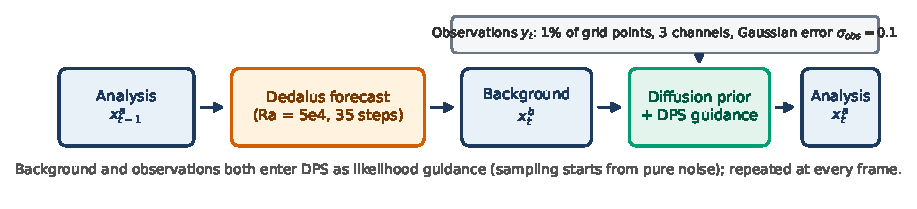
\includegraphics[width=\linewidth]{report_fig_final/workflow.pdf}\caption{循环同化流程。}\end{figure}

\subsection{DPS 后验采样中的引导项}
记 $\hat x_0(x_t)$ 为网络对干净场的估计。每步采样在先验得分上叠加三类引导：观测项 $\|y-H\hat x_0\|^2/2\sigma_{\rm obs}^2$（$\sigma_{\rm obs}=0.05$）；背景项 $\|x^b-\hat x_0\|^2/2\sigma_{\rm bg}^2$（$\sigma_{\rm bg}=0.3$，$x^b$ 为求解器预报）；散度惩罚 $\lambda\sum(\nabla\!\cdot u(\hat x_0)/G)^2$（$\lambda=0.3$，谱导数，$G$ 为真值初始场梯度的均方根）。总引导强度系数为 2，不对采样结果强制观测点取观测值。采样器为 ODE-DPM1，100 步，起始时刻 $t=0.4$，每窗口 32 个样本，取样本均值为分析场。$\sigma_{\rm obs}$ 是引导强度，并不等同于观测噪声标准差（验证集最优 0.05 小于真实噪声 0.1，原因未明）。

\subsection{无散度、无滑移投影（A1）}
采样输出不保证 $\nabla\!\cdot u=0$。我们把速度投影到由流函数导出的子空间：$u=(\partial_z\psi,-\partial_x\psi)$，$\psi$ 与 $\partial_z\psi$ 在真实壁面（$z=0,L_z$）为零；基函数为带壁面包络的 16 个模态，导数矩阵与散度诊断使用的 Chebyshev 谱导数一致，$b$ 通道不动。float64 下投影后散度为 $10^{-15}$，真壁面速度为 $10^{-14}$，投影对称幂等，对真值本身只改动约 0.2\%。\textbf{A1} 即对每个后验样本采样完后投影一次，投影后的场进入下一循环。

\subsection{循环流程}
循环 $t=0,1,\dots$：$t=0$ 无背景，仅由观测引导采样；$t>0$ 时用 Dedalus 求解器把上一次分析预报到当前时刻作为背景。每隔 $K$ 帧同化一次，其余帧直接取预报状态；第 0 帧一定同化。求解器取 Ra$=5\times10^4$，数据真值为 $10^5$，由此制造模型误差。

\subsection{基线：随机 EnKF}
20 个成员，每个成员的观测叠加独立扰动，$R=0.01\,I$（标准差 0.1），乘性膨胀 1.1（$K=20,50$ 时用验证集上最优的 1.4），不使用局地化，预报模型与 A1 相同。初始集合不能全取同一状态：此时集合协方差为零、增益为零，观测不起作用。初始集合以 A1 的第 0 帧分析为中心，叠加去均值（集合均值严格等于中心）的物理一致扰动（$b$ 乘壁面包络，速度由流函数一次缩放得到，幅度为参考标准差的 0.1 倍），并跳过自身的 $t=0$ 更新。另一种构造是取 20 个互不相同的真实流场作初始集合，验证轨迹上稳态误差相同（0.0250），故采用前者。

\section{实验设置}
\begin{table}[H]\centering\small\caption{误差来源与取值。}
\begin{tabular}{p{2.1cm}p{2.3cm}p{7.6cm}}\toprule
类别 & 作用对象 & 设定\\\midrule
观测噪声 & 观测值 & 零均值高斯，标准差 0.1（三通道相同），每个同化帧独立重抽；同一轨迹、同一种子下三种方法看到相同的观测与噪声\\
观测稀疏性 & 观测位置 & 1\% 格点（17/1728），三通道同时观测，位置由种子决定、同轨迹内固定\\
模型误差 & 求解器预报 & 预报 Ra$=5\times10^4$，真值 $10^5$；每步预报累积，是同化要纠正的主要误差\\
初始状态误差 & 第 0 帧 & 无背景，仅由该帧稀疏噪声观测经 DPS 得到，不用真值作初值\\\bottomrule
\end{tabular}\end{table}
数据：训练/验证/测试 160/20/20 个轨迹，每轨迹 100 帧。观测间隔 $K=1,20,50$（$K=20$ 时第 0、20、40、60、80 帧同化，$K=50$ 时第 0、50 帧同化）。指标为未观测点 RMSE（100 帧平均）与相对散度 $\|\nabla\!\cdot u\|/\|\nabla u\|$（谱导数；真值约 $3.5\times10^{-5}$），散度同时报告保存分析场的``原始''值与施加同一投影后的值。随机种子同时决定观测位置、噪声、采样噪声与 EnKF 初始扰动；主结果在种子 42、43、44 上各跑一遍。\textbf{超参数只在验证轨迹上选择，测试轨迹仅用于最终评估。}

\section{结果}
\subsection{主结果}
\begin{table}[H]\centering\small\caption{测试集 20 个轨迹的未观测点 RMSE（种子 42 / 43 / 44）。EnKF 在 $K=1$ 用膨胀 1.1，$K=20,50$ 用 1.4。}
\resizebox{\linewidth}{!}{\begin{tabular}{cccccc}\toprule
$K$ & A1 & EnKF & 纯预报 & A1 误差降低 & A1 更优轨迹数\\\midrule
1 & 0.0161 / 0.0162 / 0.0158 & 0.0264 / 0.0268 / 0.0257 & 0.0488 / 0.0462 / 0.0462 & 39.0\% / 39.7\% / 38.5\% & 20/20 / 20/20 / 20/20 \\
20 & 0.0372 / 0.0375 / 0.0354 & 0.0417 / 0.0407 / 0.0390 & 0.0488 / 0.0462 / 0.0462 & 10.8\% / 7.9\% / 9.5\% & 18/20 / 17/20 / 17/20 \\
50 & 0.0442 / 0.0434 / 0.0425 & 0.0472 / 0.0453 / 0.0448 & 0.0488 / 0.0462 / 0.0462 & 6.4\% / 4.1\% / 5.1\% & 19/20 / 18/20 / 18/20 \\
\bottomrule\end{tabular}}\end{table}
\begin{figure}[H]\centering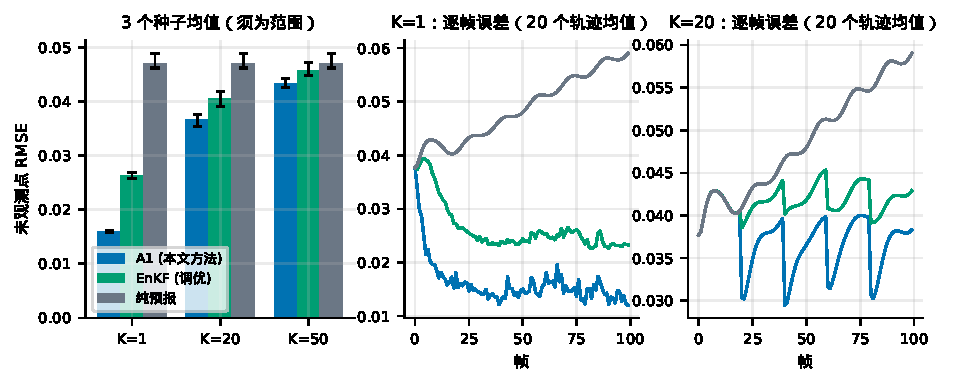
\includegraphics[width=\linewidth]{report_fig_final/main.pdf}\caption{左：三种方法在各观测间隔下的 RMSE；中、右：$K=1$ 与 $K=20$ 的逐帧误差（种子 42）。}\end{figure}
$K=1$ 时 A1 比 EnKF 低约 39\%，三个种子的 60 个轨迹次全部更优，与验证集上的相对优势（38\%）一致，说明参数未对验证集过拟合。间隔增大时两种方法都向纯预报靠拢（观测稀疏时误差主要由 Rayleigh 数失配造成的预报漂移决定），A1 的优势缩小到约 9\%（$K=20$）与 5\%（$K=50$），每个种子里有 1--3 个轨迹 A1 不占优，该区间内只能表述为``略优''。EnKF 的膨胀系数影响明显：$K=20$ 时由 1.1 换为 1.4，EnKF 误差由 0.0452 降到 0.0417；$K=1$ 时 1.4 反而更差（0.0347 对 0.0264）。

\begin{figure}[H]\centering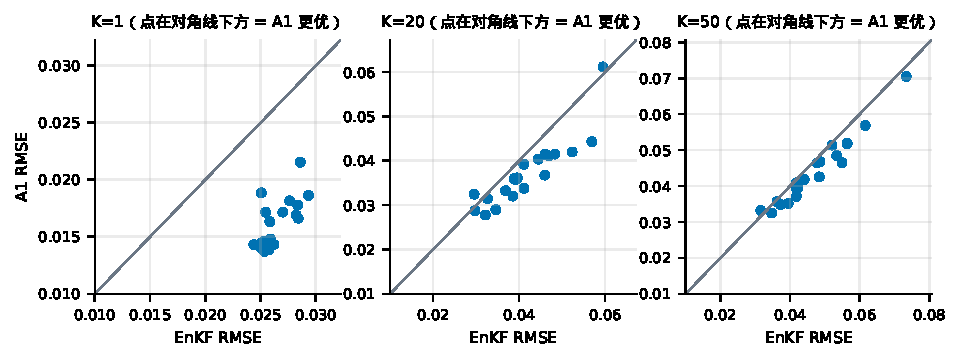
\includegraphics[width=\linewidth]{report_fig_final/cases.pdf}\caption{逐轨迹配对比较（种子 42）。}\end{figure}

\subsection{散度}
\begin{table}[H]\centering\small\caption{相对散度（种子 42，20 个轨迹均值；EnKF 膨胀 1.1）。}
\begin{tabular}{ccccc}\toprule
$K$ & 方法 & 原始 & 同一投影后\\\midrule
1 & A1 & $4.2\times10^{-7}$ & $1.2\times10^{-7}$ \\
1 & EnKF & $9.5\times10^{-6}$ & $1.3\times10^{-7}$ \\
1 & 纯预报 & $9.1\times10^{-6}$ & $1.3\times10^{-7}$ \\
20 & A1 & $9.6\times10^{-6}$ & $1.3\times10^{-7}$ \\
20 & EnKF & $9.0\times10^{-6}$ & $1.3\times10^{-7}$ \\
20 & 纯预报 & $9.1\times10^{-6}$ & $1.3\times10^{-7}$ \\
50 & A1 & $9.3\times10^{-6}$ & $1.3\times10^{-7}$ \\
50 & EnKF & $9.0\times10^{-6}$ & $1.3\times10^{-7}$ \\
50 & 纯预报 & $9.1\times10^{-6}$ & $1.3\times10^{-7}$ \\
\bottomrule\end{tabular}\end{table}
$K=1$ 时 A1 的原始散度比 EnKF 低约一个数量级，是因为 A1 在保存前已做投影而 EnKF 没有；\textbf{对分析场施加同一投影后两者相同}。$K=20,50$ 时多数帧是求解器的预报输出，原始散度处于求解器输出自身水平，两种方法无区别。因此在不可压缩约束上，本文的结论是：A1 交付的场满足物理约束且无精度损失，在投影口径下与 EnKF 持平，而不是更优。验证轨迹上的消融（5 个轨迹，$K=1$）显示：不投影时 RMSE 0.0158、保存场散度 $4.2\times10^{-2}$；投影后 0.0157、$4.2\times10^{-7}$；去掉散度惩罚（$\lambda=0$）在 5/5 个轨迹上更差。

\subsection{对模型误差的稳健性}
\begin{table}[H]\centering\small\caption{改变预报 Ra 的未观测点 RMSE（$K=1$，20 个轨迹，种子 42；参数未重调）。}
\begin{tabular}{cccccc}\toprule
预报 Ra & A1 & EnKF & 纯预报 & A1 更优轨迹数\\\midrule
1e5 & 0.0169 & 0.0150 & 0.0425 & 1/20 \\
8e4 & 0.0166 & 0.0163 & 0.0427 & 9/20 \\
5e4 & 0.0161 & 0.0264 & 0.0488 & 20/20 \\
2e4 & 0.0160 & 0.0548 & 0.0668 & 20/20 \\
\bottomrule\end{tabular}\end{table}
\begin{figure}[H]\centering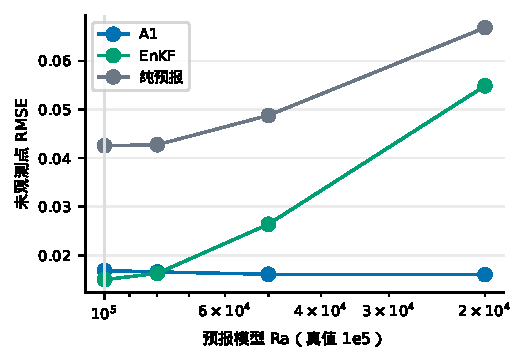
\includegraphics[width=.55\linewidth]{report_fig_final/ra.pdf}\caption{RMSE 随预报模型失配的变化。}\end{figure}
A1 的误差基本不随失配变化，EnKF 随失配增大急剧变差（Ra$=2\times10^4$ 时已接近纯预报）。预报模型准确（Ra$=10^5$）时 EnKF 更好，$8\times10^4$ 附近持平，$5\times10^4$ 及以下 A1 更好。因此优势应表述为\textbf{对模型误差稳健}，而不是任何条件下都更准。A1 的参数在 $5\times10^4$ 下选定，无失配时略逊于 EnKF 可能与此有关，未重调验证。

\subsection{初值误差的恢复}
第 0 帧给出远离真值的初始猜测，之后每帧同化（$K=1$，10 个测试轨迹，种子 42，参数不重调）。A1 把猜测作为第 0 帧背景；EnKF 以它为中心且第 0 帧也同化；纯预报从它出发。``恢复帧数''为未观测点 RMSE 首次低于 0.03 的帧号（轨迹中位数）。
\begin{table}[H]\centering\scriptsize\caption{坏初值的恢复。}
\begin{tabular}{lccccccc}\toprule
初始猜测 & 初值 RMSE & \multicolumn{3}{c}{恢复帧数} & \multicolumn{3}{c}{100 帧平均 RMSE}\\
 & & A1 & EnKF & 纯预报 & A1 & EnKF & 纯预报\\\midrule
全 0 & 0.352 & 3.5 & 55 & 未恢复 & 0.0171 & 0.0740 & 0.2177 \\
真值的 0.3 倍 & 0.246 & 1 & 48 & 未恢复 & 0.0159 & 0.0545 & 0.1009 \\
另一时刻（第 60 帧） & 0.050 & 1.5 & 10 & 37 & 0.0159 & 0.0264 & 0.0352 \\
真值 + 100\% 噪声 & 0.148 & 1.5 & 31 & 未恢复 & 0.0158 & 0.0354 & 0.0755 \\
真值 + 200\% 噪声 & 0.296 & 5 & 41 & 未恢复 & 0.0168 & 0.0506 & 0.1256 \\
\bottomrule\end{tabular}\end{table}
\begin{figure}[H]\centering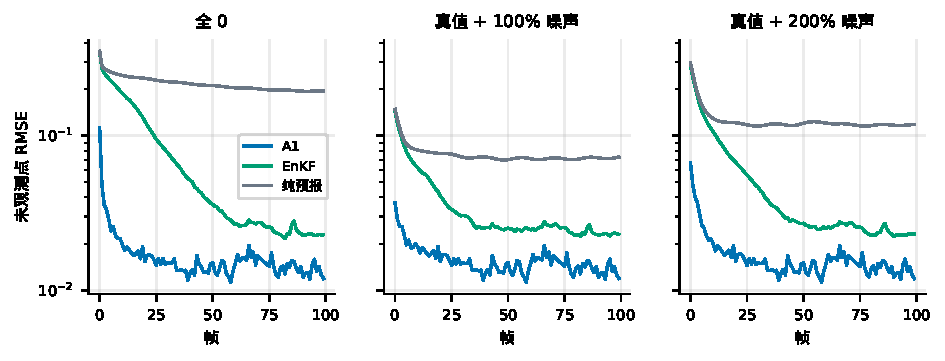
\includegraphics[width=\linewidth]{report_fig_final/init.pdf}\caption{坏初值下的逐帧 RMSE（10 个轨迹均值，纵轴对数）。}\end{figure}
A1 在 1--5 帧内恢复，EnKF 需 10--55 帧；纯预报对多数初值不能恢复，因为 RB 流动变化缓慢，初值误差衰减很慢。

\subsection{EnKF 集合离散度的演化}
\begin{table}[H]\centering\small\caption{EnKF 的 spread 与集合均值误差（测试轨迹 0--4，种子 42）。}
\begin{tabular}{cccccc}\toprule
$K$ & 膨胀 & 第 0 帧 spread & 第 0 帧误差 & 第 50--99 帧 spread & 第 50--99 帧误差\\\midrule
1 & 1.1 & 0.0143 & 0.0380 & 0.0149 & 0.0242 \\
20 & 1.1 & 0.0143 & 0.0380 & 0.0067 & 0.0484 \\
20 & 1.4 & 0.0143 & 0.0380 & 0.0121 & 0.0437 \\
50 & 1.4 & 0.0143 & 0.0380 & 0.0072 & 0.0504 \\
\bottomrule\end{tabular}\end{table}
\begin{figure}[H]\centering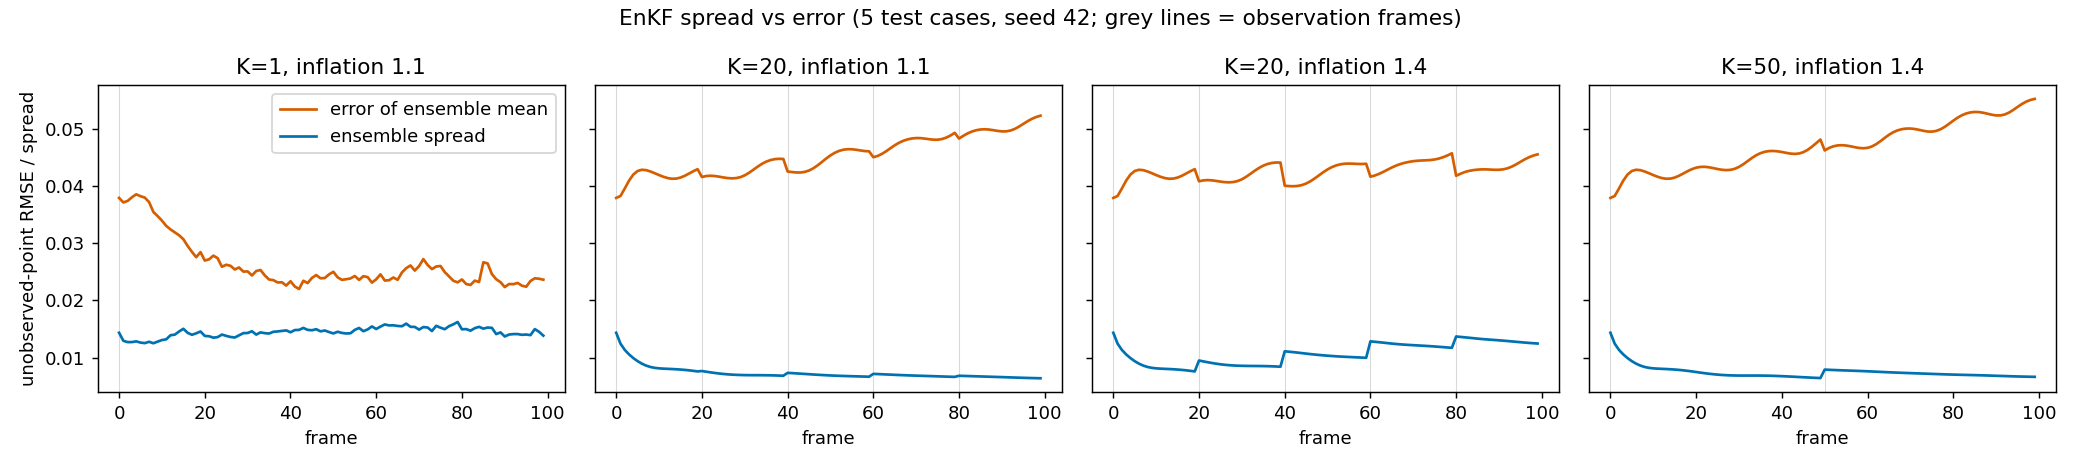
\includegraphics[width=\linewidth]{report_fig_final/spread.png}\caption{spread 与误差随帧的变化（灰线为观测帧）。}\end{figure}
初始 spread 约 0.014，而第 0 帧误差约 0.038，初始集合本身偏自信。$K=1$ 时每帧同化使 spread 稳定在 0.013--0.015，约为误差的 0.6 倍；观测间隔变长时，观测之间的纯预报使 spread 逐渐收缩而误差增长，集合越来越偏自信，增益变小，修正不足。增大膨胀能抬高稳态 spread（$K=20$：0.0067 到 0.0121），对应误差更低，这是长间隔下 1.4 更优的一个解释；该解释来自数字对照，未做严格的 spread--skill 诊断，且仅基于 5 个轨迹、单一种子。

\subsection{未带来收益的尝试}
加数据与加大先验（训练轨迹增至 560、通道数加宽到 32）使验证损失由 0.0435 降至 0.0284 与 0.0251，但验证轨迹上的循环 RMSE 反而由 0.0167 变为 0.0179 与 0.0197，原因未查明；软化观测权重在单步上有效（0.0099$\to$0.0052）却在循环中变差；增大散度惩罚（$\lambda\ge1$）变差或发散。结论：先验与引导的改进必须在循环中验证，单步结果会误导。

\section{局限}
\begin{enumerate}
\item 主结果为 3 个种子、每个种子 20 个轨迹；3 个种子仍不足以给出严格的方差估计。Ra 与坏初值实验为单种子，后者只有 10 个轨迹，spread 实验只有 5 个轨迹。
\item EnKF 的膨胀只在 $\{1.0,1.1,1.2,1.4\}$ 与两种局地化中扫描，更大的膨胀、成员数与初始扰动幅度没有系统扫描，长间隔下的 EnKF 可能仍有改进余地。
\item A1 与 EnKF 的参数在 Ra$=5\times10^4$ 的失配下选定，Ra 与坏初值实验沿用而未重调。
\item 只考察观测噪声 0.1，未做噪声水平扫描；$\sigma_{\rm obs}$ 最优值小于真实噪声的原因未明；个别轨迹上 A1 的优势明显更小，原因未查。
\item 求解器预报代码把最靠近壁面的内部节点速度置零，而真实壁面不在配点上，该处理的影响未单独核查；不做投影直接重启求解器是否变差，没有对照数据。
\item 仅在 RB 上完成完整对比。
\end{enumerate}
\end{document}
